% main.tex

\documentclass{beamer}

\usepackage{template/Politecnico-di-Torino-Presentation/beamerthemesintef} % updated path
\usepackage{amsfonts,amsmath,oldgerm}

\usetheme{sintef}

\newcommand{\testcolor}[1]{\colorbox{#1}{\textcolor{#1}{test}}~\texttt{#1}}
\usefonttheme[onlymath]{serif}
\titlebackground*{template/Politecnico-di-Torino-Presentation/assets/background} % updated path
\newcommand{\hrefcol}[2]{\textcolor{cyan}{\href{#1}{#2}}}

\usepackage{listings}
\usepackage{xcolor}
\usepackage{hyperref}

\lstset{
    basicstyle=\ttfamily\footnotesize,
    keywordstyle=\color{blue},
    commentstyle=\color{gray},
    stringstyle=\color{red},
    % numbers=left,
    % numberstyle=\tiny\color{gray},
    % stepnumber=1,
    % numbersep=5pt,
    showstringspaces=false,
    breaklines=true,
    frame=single,
    tabsize=4,
    language=C
}

% Presentation info
\title{Secure Timeout System \newline NXP S32K3X8EVB}
\subtitle{Beamer for the CAOS Project}
\author{
    \newline Andrea Botticella
    \newline Fabrizio Emanuel 
    \newline Elia Innocenti
    \newline Renato Mignone 
    \newline Simone Romano     
}
\date{February 5, 2025}

% Begin document
\begin{document}
\maketitle

% Include the sections of the presentation
% 01-overview.tex

\section{Project Overview}

\begin{frame}{Project Overview}
    \begin{itemize}
        \item Implement a secure timeout system application on the NXP S32K3X8EVB board using FreeRTOS, emulated with QEMU.
        \item Divided into several parts, each focusing on different aspects of the development process.
    \end{itemize}
\end{frame}

\section{Projects’ Goal}

\begin{frame}{Projects’ Goal}
    \begin{itemize}
        \item Learn how to use different technologies:
        \begin{itemize}
            \item QEMU to emulate a heterogeneous hardware architecture.
            \item FreeRTOS for real-time operating system functionalities.
        \end{itemize}
        \item Learn how to use Git to manage a team project:
        \begin{itemize}
            \item Efficient collaboration and version control.
        \end{itemize}
        \item Learn how to present your work:
        \begin{itemize}
            \item Documenting and presenting the project effectively.
        \end{itemize}
    \end{itemize}
\end{frame}

% 02-qemu-emulation.tex

\section{QEMU Board Emulation}

\begin{frame}{Custom QEMU Version}
    \begin{itemize}
        \item Emulate the NXP S32K3X8EVB board, which is not natively supported by QEMU.
        \item Ensure proper emulation of the CPU (ARM Cortex-M7), memory map, and peripherals.
    \end{itemize}
\end{frame}

\begin{frame}{Technical Details}
    \begin{itemize}
        \item Added a new machine model to QEMU for the S32K3X8EVB board.
        \item Used previous QEMU implementations as reference (ARMv7-M architecture).
        \item Implemented custom initialization routines for memory and peripherals.
        \item S32K358EVB board has the following specification:
            \begin{itemize}
                \item ARM Cortex-M7 CPU.
                \item \(\sim \)8MB Flash memory, 768KB SRAM, 256KB DTCM, and 128KB ITCM.
                \item NVIC with 256 IRQs and 4 priority bits.
                \item Multiple peripherals: 16 LPUART, 3 PIT timers, 16 MPU regions.
                \item System clock running at 240MHz.
            \end{itemize}
    \end{itemize}
\end{frame}

\begin{frame}{Memory Regions Initialization}
    \begin{itemize}
        \item \textbf{Flash Memory}: Configured multiple blocks:
        \begin{itemize}
            \item Block0: Base Address: 0x00400000, Size: 2 MB
            \item Block1: Base Address: 0x00600000, Size: 2 MB
            \item Block2: Base Address: 0x00800000, Size: 2 MB
            \item Block3: Base Address: 0x00A00000, Size: 2 MB
            \item Block4: Base Address: 0x10000000, Size: 128 KB
            \item Utest: Base Address: 0x18000000, Size: 8 KB
        \end{itemize}
        \item \textbf{SRAM Memory}:
        \begin{itemize}
            \item Block0: Base Address: 0x20400000, Size: 256 KB
            \item Block1: Base Address: 0x20440000, Size: 256 KB
            \item Block2: Base Address: 0x20480000, Size: 256 KB
        \end{itemize}
        \item \textbf{DTCM and ITCM Memory}:
        \begin{itemize}
            \item DTCM0: Base Address: 0x20000000, Size: 128 KB
            \item ITCM0: Base Address: 0x00000000, Size: 64 KB
        \end{itemize}
    \end{itemize}
\end{frame}

\begin{frame}{Peripherals and Interrupts Setup}
    \begin{itemize}
        \item \textbf{NVIC (Nested Vectored Interrupt Controller)}:
        \begin{itemize}
            \item Configured with 256 IRQs and 4 priority bits.
            \item Interrupt vectors mapped in system memory.
        \end{itemize}
        \item \textbf{LPUART (Low Power UART)}:
        \begin{itemize}
            \item Base Address: 0x4006A000
            \item The board has \textbf{16 LPUART instances}.\\ They are mapped starting from the UART base address. 
            \item Connected to NVIC and clocked by \texttt{AIPS\_PLAT\_CLK} and \texttt{AIPS\_SLOW\_CLK}.
        \end{itemize}
        \item \textbf{PIT Timers (Periodic Interrupt Timer)}:
        \begin{itemize}
            \item Timer1: Base Address: 0x40037000
            \item Timer2: Base Address: 0x40038000
            \item Timer3: Base Address: 0x40039000
        \end{itemize}
        \item \textbf{MPU}: 16 regions.
    \end{itemize}
\end{frame}

\begin{frame}{System Clocks and Interrupts}
    \begin{itemize}
        \item \textbf{System Clock}:
        \begin{itemize}
            \item Primary System Clock: 240MHz frequency, 4.16ns period.
            \item AIPS Platform Clock: 80MHz
            \item AIPS Slow Clock: 40MHz
            %\item Reference Clock: 1MHz
        \end{itemize}
        \item \textbf{Interrupt Handling}:
        \begin{itemize}
            \item Configured NVIC to handle exceptions and IRQs.
            \item Supports up to 256 IRQs with 4 priority levels.
            \item NVIC is connected to system and reference clocks.
            %\item Bit-band support enabled for efficient memory access.
            \item Interrupt sources include timers, UARTs, and peripheral events.
        \end{itemize}
    \end{itemize}
\end{frame}

\begin{frame}{Firmware Loading}
    \begin{itemize}
        \item Function: \texttt{s32k3x8\_load\_firmware}
        \item Parameters:
        \begin{itemize}
            \item \texttt{cpu}: The ARM CPU instance.
            \item \texttt{ms}: The machine state.
            \item \texttt{flash}: The memory region representing the flash memory.
            \item \texttt{firmware\_filename}: The filename of the firmware to be loaded.
        \end{itemize}
        \item Functionality:
        \begin{itemize}
            \item Reads the firmware file and loads its contents into the specified flash memory region.
        \end{itemize}
    \end{itemize}
\end{frame}

\begin{frame}[fragile]{Class initialization}
    \begin{itemize}
    \item \texttt{s32k3x8\_class\_init}:
        \begin{lstlisting}[language=C]
static void s32k3x8_class_init(ObjectClass *oc, void *data) {
    MachineClass *mc = MACHINE_CLASS(oc);
    mc->name = g_strdup("s32k3x8evb");
    mc->desc = "NXP S32K3X8 EVB (Cortex-M7)";
    mc->init = s32k3x8_init;
    mc->default_cpu_type = ARM_CPU_TYPE_NAME("cortex-m7");
    mc->default_cpus = 1;
    mc->min_cpus = mc->default_cpus;
    mc->max_cpus = mc->default_cpus;
    mc->no_floppy = 1;
    mc->no_cdrom = 1;
    mc->no_parallel = 1;
}
        \end{lstlisting}
    \end{itemize}

\end{frame}



\section{Part 2 - FreeRTOS Porting}

\begin{frame}{FreeRTOS on Emulated Board}
    \begin{itemize}
        \item Port FreeRTOS to run on the emulated NXP S32K3X8EVB board.
        \item Ensure compatibility and functionality of FreeRTOS on the emulated hardware.
    \end{itemize}
\end{frame}

\begin{frame}{Implementation Details}
    \begin{itemize}
        \item Kernel Configuration:
        \begin{itemize}
            \item Configure FreeRTOS kernel settings in FreeRTOSConfig.h.
            \item Define task priorities, stack sizes, and heap sizes.
            \item Enable necessary FreeRTOS features like mutexes, semaphores, and task notifications.
        \end{itemize}
    \end{itemize}
\end{frame}

% 04-application.tex

\section{Part 3 - Write a Simple Application}

\begin{frame}{Secure Timeout System Application}
    \begin{itemize}
        \item The application is a simple implementation of a \textit{Secure Timeout System}.
        \item It consists of \textbf{multiple tasks} that simulate events, monitor activities, and handle alerts.
        \item \textbf{Hardware timers} are used to generate \textbf{periodic interrupts} for activity detection.
    \end{itemize}
\end{frame}

\begin{frame}{Task Implementation}
    \begin{itemize}
        \item \textbf{Event Task:}
            \begin{itemize}
                \item Periodically generates events that can be either user activities or suspicious activities.
                \item Uses a pseudo-random number generator to decide the type of event.
                \item Logs the generated event and updates the respective counters.
            \end{itemize}
    \end{itemize}
    \begin{figure}[h]
        \centering
        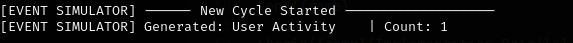
\includegraphics[width=0.75\textwidth]{images/event_task_1.png}
    \end{figure}
    \begin{figure}[h]
        \centering
        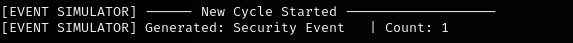
\includegraphics[width=0.75\textwidth]{images/event_task_2.png}
        \caption{Generation of a user activity and a suspicious activity.}
    \end{figure}
\end{frame}

\begin{frame}{Hardware Timer Initialization}
    \begin{itemize}
        \item \textbf{Timer 0:}
            \begin{itemize}
                \item Configured to generate periodic interrupts.
                \item Interrupt handler checks for \textbf{user activities} and sets the user activity detection flag.
            \end{itemize}
        \item \textbf{Timer 1:}
            \begin{itemize}
                \item Configured to generate periodic interrupts.
                \item Interrupt handler checks for \textbf{suspicious activities} and sets the suspicious activity detection flag.
            \end{itemize}
    \end{itemize}
\end{frame}

\begin{frame}{Task Implementation}
    \begin{itemize}
        \item \textbf{Monitor Task:}
            \begin{itemize}
                \item Checks for user activity detection.
                \item Logs the status of user activity.
                \item Resets the user activity detection flag after logging.
            \end{itemize}
        \item \textbf{Alert Task:}
            \begin{itemize}
                \item Checks for suspicious activity detection.
                \item Logs the status of the system security.
                \item Initiates security protocols if suspicious activity is detected.
                \item Resets the suspicious activity detection flag after logging.
            \end{itemize}
    \end{itemize}
\end{frame}

\begin{frame}{Implementation Details}
    \begin{itemize}
        \item \textbf{Global Variables:}
            \begin{itemize}
                \item Four main \textbf{flags}:
                    \begin{itemize}
                        \item \texttt{userActivity}, \texttt{userActivityDetection}, \\ \texttt{suspiciousActivity}, \texttt{suspiciousActivityDetection}
                    \end{itemize}
            \end{itemize}
        \item \textbf{Task Priorities:}
            \begin{itemize}
                \item Event Task has the highest priority to ensure timely event generation.
                \item Monitor Task and Alert Task have lower priorities.
            \end{itemize}
        \item \textbf{Timer Frequency:}
            \begin{itemize}
                \item Timer 0 and Timer 1 are configured to generate periodic interrupts \\at a frequency of 2 Hz.
            \end{itemize}
    \end{itemize}
\end{frame}

\begin{frame}[fragile]{Implementation Details}
    \begin{itemize}
        \item \textbf{Task Priorities:}
            \begin{lstlisting}[language=C]
// filepath: /App/SecureTimeoutSystem/secure_timeout_system.c
#define MONITOR_TASK_PRIORITY (tskIDLE_PRIORITY + 2)
#define ALERT_TASK_PRIORITY   (tskIDLE_PRIORITY + 3)
#define EVENT_TASK_PRIORITY   (tskIDLE_PRIORITY + 4)
            \end{lstlisting}
        \item \textbf{Timer Frequency:}
            \begin{lstlisting}[language=C]
// filepath: /App/Peripherals/IntTimer.c
#define tmrTIMER_0_FREQUENCY (2UL)
#define tmrTIMER_1_FREQUENCY (2UL)
            \end{lstlisting}
    \end{itemize}
\end{frame}

\begin{frame}{Run Example}
    \begin{figure}[h]
        \centering
        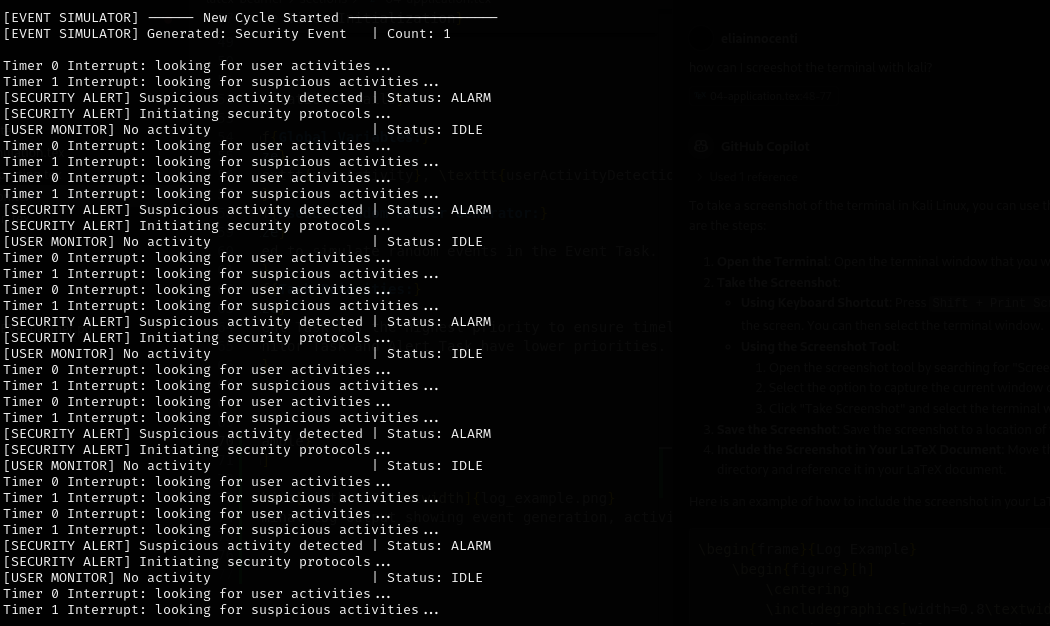
\includegraphics[width=0.75\textwidth]{images/run_example.png}
        % \caption{Terminal log output showing event generation, activity detection, and alert handling.}
    \end{figure}
\end{frame}

\section{Conclusion}

\begin{frame}{Conclusion}
    \begin{itemize}
        \item The s32k3x8evb\_board.c file plays a crucial role in the emulation of the NXP S32K3X8EVB board within QEMU.
        \item It provides the necessary functions to load firmware, initialize memory regions, set up hardware components, and manage system clocks and interrupts.
        \item This detailed analysis highlights the key functionalities and their implementations, providing a comprehensive understanding of the board initialization and configuration process.
    \end{itemize}
\end{frame}


\title{} % Reset the title to have a better backmatter visualization
\backmatter

\end{document}
